\documentclass[12pt,a4paper]{article}
\usepackage[utf8]{inputenc}
\usepackage{graphicx}
\usepackage{hyperref}
\usepackage{multirow}
\usepackage{booktabs}
\renewcommand{\baselinestretch}{1.2}
\title{Analyzing King Saud University Computer Science Curriculum}
\author{Mohand Alrasheed}
\date{2022 / January}

\begin{document}
\pagenumbering{gobble}

\maketitle
\clearpage

\tableofcontents
\clearpage


\section{Introduction}
King Saud University's computer science curriculum has many pros and cons, in this document we outline a criteria for judging courses and ranking the curriculum based on experts' opinions.

\section{Assumptions} 
We make a number of assumptions regarding the evaluation of courses, these guide the evaluation process so they should be read carefully before moving on to results.

\paragraph{Assumptions}
\begin{enumerate}
    \item The course instructor's influence is minimized when ranking courses by imagining all courses being taught by a perfect instructor.
    \item The ranking has been chosen by students mostly on their final semester, which would mean most of them have not studied the last semester and in turn we will not take its courses into consideration in this version.
    \item The ranking has been chosen by students mostly belonging batch 439 and 438, different batches might rank courses differently as co\textbf{}urse content changes slowly.
    \item Most electives are not taken into consideration, but a small number of popular electives will be considered. 
\end{enumerate}

\section{Criteria}
Courses are judged based on five criteria chosen by the most elite members of 439.

\paragraph{Criteria}
\begin{enumerate}
    \item \textbf{Applications}: This refers to real-world applications of the knowledge gained by studying the course.
    \item \textbf{Relevance}: This refers to the new-ness of the knowledge taught compared to the current (as of this document's date) state of the art.
    \item \textbf{Insight}: This refers to the quality of the knowledge gained with respect to understanding the world and expanding one's horizons.
    \item \textbf{Understanding}: This refers to the proportion of the course's understanding portions over the memorization portions. 
    % \item \textbf{Completeness}: This refers to how connected the course is as a package. A course with randomly assembled useful info will score badly on this category, while a cohesively assembled useless info scores highly.
    \item \textbf{Ease}: This refers to how easy the course was.
\end{enumerate}

\section{Method}
\subsection{Data}
The data is collected and sorted using \emph{Google Forms} in which each reviewer identifies their university batch and sex as well as rate an optional number of courses, i.e. the reviewer can review zero courses, or all courses if they wish. Each reviewer can optionally also provide extra notes alongside any course. 

The number of courses ended up being 42, where we include the core plan as well as popular electives. We end up with a number of reviewers totaling 16 reviewers where the minimum number of reviews per course is 2 and the maximum is 14, the distribution of counts is skewed to the right where the 50th percentile is 11 and the 75th is 13. After collecting the data we end up with (Courses, Criteria) X Reviewer matrix.

\subsection{Score calculation}
Due to the low sample size on reviews of some courses we treat the problem as a \emph{Bayesian estimation} problem. In our implementation we possess an idea of the original values we're predicting what we call the \emph{prior}, which in this case will be the arithmetic mean of a criterion on some category\footnote{Categories are divided in this way: Humanities, Mathematics, Chemistry, Islamics, Physics, Computer science}, then we  update our beliefs given new evidence (reviews) by taking a weighted average of the criterion and the prior. \[(r_1 * w_1 + .. + r_n * w_n + c{_m_e_a_n} * w_c)/(\Sigma^n_{i_=_1} w_i + w_c)\]
We experimented with the weight of the category mean \(c_{m_e_a_n}\) and arrived at a weight half as weighty as the weight of the reviews.

After collecting and processing the data we will rank courses using a weighted mean of criteria, we will use three different weights.

\paragraph{Weighing technique}
\begin{enumerate}
    \item \textbf{General}: This weighing takes everything into account fairly, equivalent to a traditional mean. \[Applications\; +\; Relevance\; +\; Insight\; +\; Understanding\; +\; Ease\]
    \item \textbf{Real-world}: This score mainly focuses on real world utility. \[Applications * 1.5\; +\; Relevance\; +\; Insight * 0\; +\; Understanding * 0.2\; +\; Ease * 0.5\]
    \item \textbf{Academic}: This score only focuses on the academic aspect of courses. \[Applications * 0\; +\; Relevance * 0\; +\; Insight * 1.5\; +\; Understanding * 1.5\; +\; Ease * 0\]
\end{enumerate}


\section{Results}
\hskip-1.7cm
\begin{tabular}{lrrrl}
\toprule
{} &  Real-world score &  Academic score &  General score &        categories \\
\midrule
ENGLISH100      &          0.977969 &        0.587055 &       0.749899 &        Humanities \\
ARB100          &          0.644273 &        0.561107 &       0.559423 &        Humanities \\
MATH101         &          0.899391 &        0.883593 &       0.772007 &       Mathematics \\
CHEM101         &          0.520728 &        0.438133 &       0.445344 &         Chemistry \\
STAT101         &          0.927789 &        0.804526 &       0.756429 &       Mathematics \\
TECH101         &          0.765262 &        0.545605 &       0.626730 &        Humanities \\
ENTREPRENEUR101 &          0.601895 &        0.521720 &       0.530546 &        Humanities \\
FAJAB101        &          0.600165 &        0.538924 &       0.546742 &        Humanities \\
NAHAJ101        &          0.638404 &        0.661528 &       0.594242 &        Humanities \\
ENGLISH110      &          0.918583 &        0.582118 &       0.713858 &        Humanities \\
SALAM107        &          0.754027 &        0.638643 &       0.659744 &          Islamics \\
PHYS104         &          0.624921 &        0.534890 &       0.519392 &           Physics \\
MATH106         &          0.794863 &        0.735696 &       0.674323 &       Mathematics \\
CSC111          &          0.984843 &        0.934987 &       0.849246 &  Computer science \\
MATH151         &          0.954951 &        0.868024 &       0.817721 &       Mathematics \\
SALAM108        &          0.634832 &        0.415596 &       0.526326 &          Islamics \\
CSC113          &          0.840633 &        0.775292 &       0.730219 &  Computer science \\
CSC220          &          0.862635 &        0.832111 &       0.739635 &  Computer science \\
MATH244         &          0.831908 &        0.716022 &       0.674008 &       Mathematics \\
CSC212          &          0.943643 &        1.000000 &       0.839300 &  Computer science \\
CSC215          &          0.801212 &        0.781024 &       0.676474 &  Computer science \\
MATH281         &          0.848302 &        0.846393 &       0.748259 &       Mathematics \\
CSC304          &          0.676360 &        0.582436 &       0.612944 &  Computer science \\
CSC380          &          0.795881 &        0.727745 &       0.676944 &  Computer science \\
CSC227          &          0.740514 &        0.637227 &       0.619513 &  Computer science \\
CSC311          &          0.993665 &        0.991418 &       0.866180 &  Computer science \\
CSC339          &          0.671742 &        0.846109 &       0.679513 &  Computer science \\
CSC343          &          0.659292 &        0.501000 &       0.529513 &  Computer science \\
CSC361          &          0.801822 &        0.819164 &       0.703416 &  Computer science \\
CSC329          &          0.971137 &        0.964173 &       0.849513 &  Computer science \\
CSC340          &          0.609492 &        0.737127 &       0.586180 &  Computer science \\
CSC453          &          0.658107 &        0.646309 &       0.582847 &  Computer science \\
CSC496          &          0.898492 &        0.796582 &       0.736309 &  Computer science \\
PHYS103         &          0.611916 &        0.635857 &       0.542905 &           Physics \\
CSC443          &          0.683071 &        0.549409 &       0.578540 &  Computer science \\
CSC462          &          1.000000 &        0.922291 &       0.843796 &  Computer science \\
CSC489          &          0.792190 &        0.732545 &       0.691387 &  Computer science \\
\bottomrule
\end{tabular}

\subsection{Visuals}
We include the most important visualizations done. Which are the general scores ranking and the weighted scores ranking. More visualization and a live demo with interact-able graphs can be found here: \href{http://courses.hawzen.me}{courses.hawzen.me}.

\begin{figure}
    \centering
    \hskip-1.7cm \rotatebox[origin=c]{90}{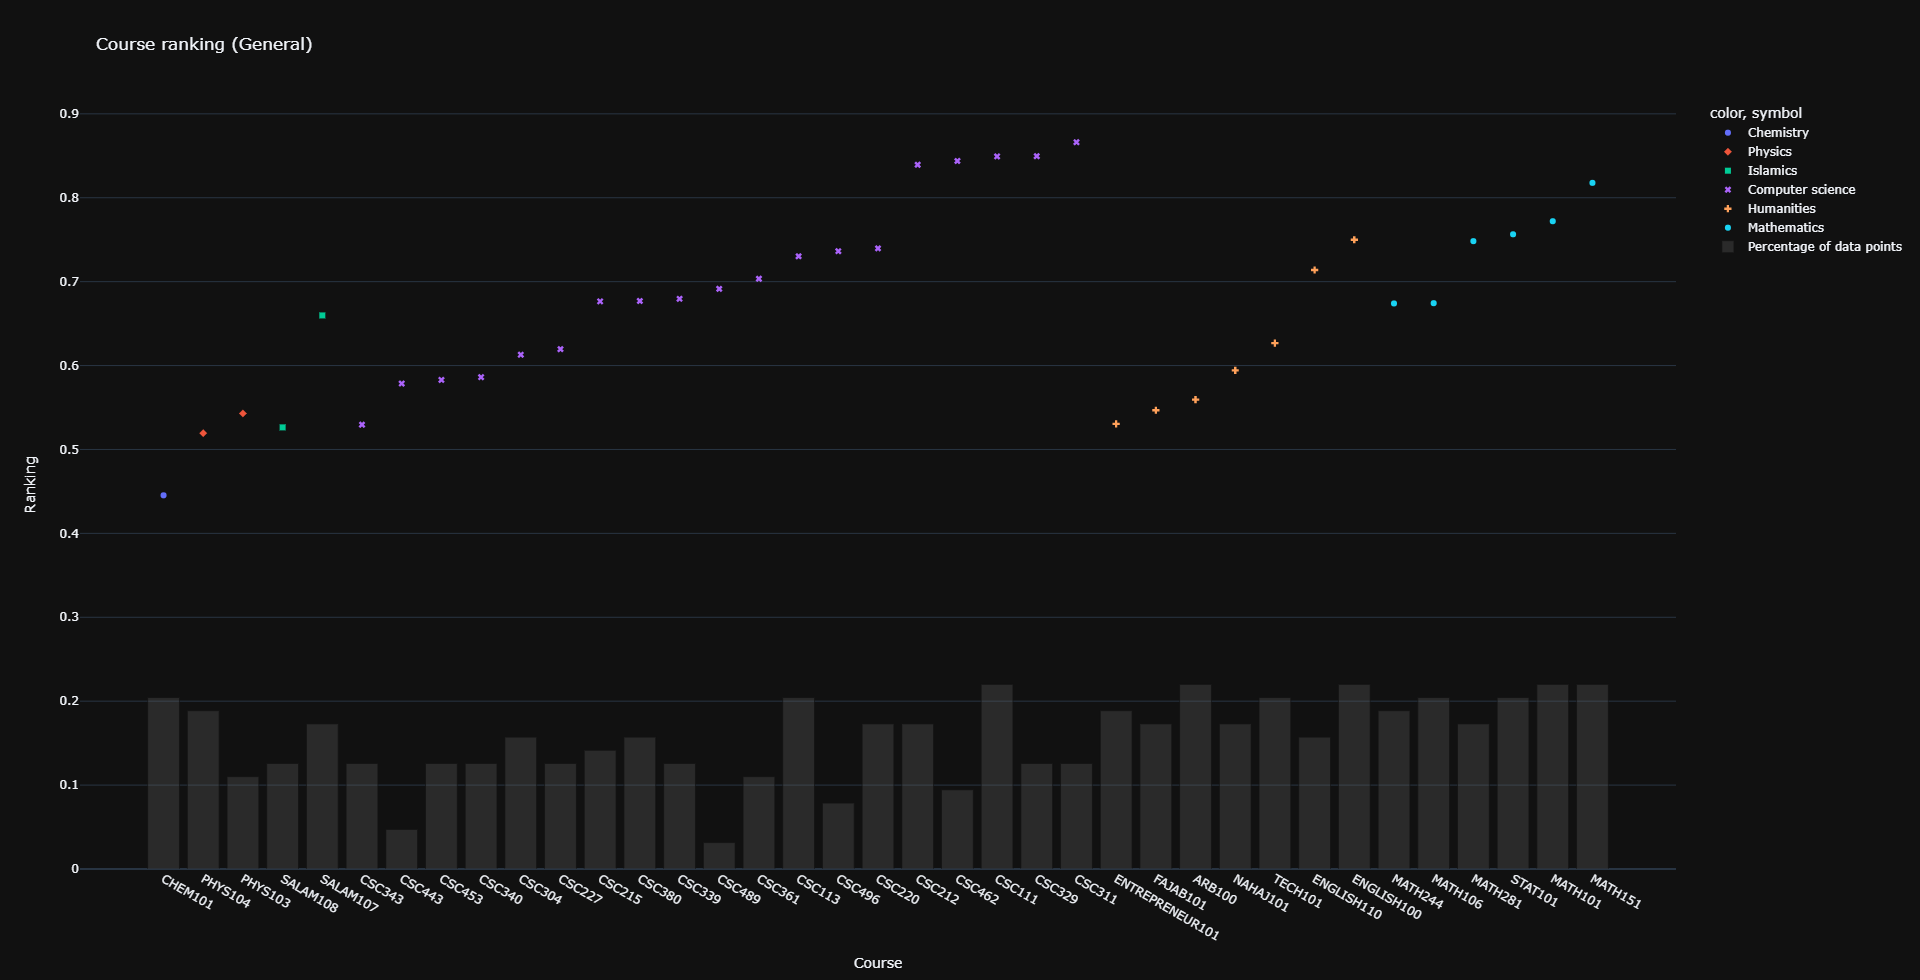
\includegraphics[scale=.3]{normal.png}}
    \caption{Scores based on general ranking}
    \label{fig:general_ranking}
\end{figure}

\begin{figure}
    \centering
    \rotatebox[origin=c]{90}{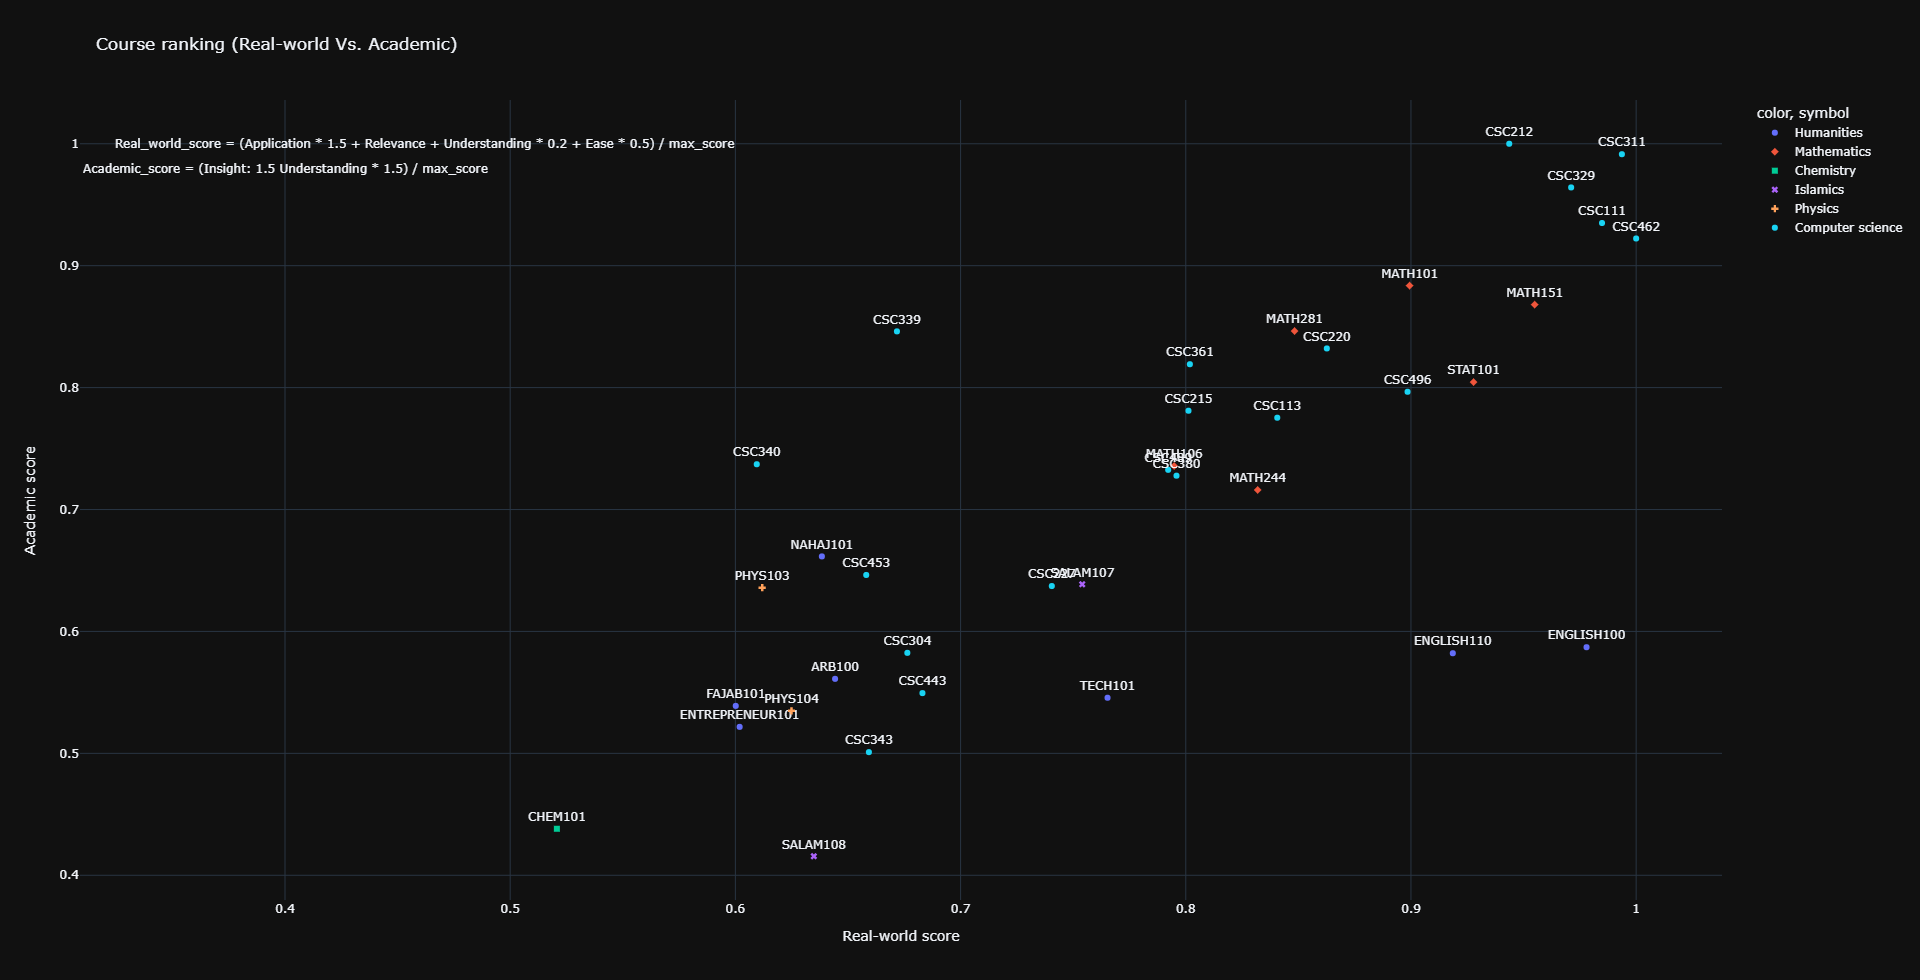
\includegraphics[scale=.3]{weighted.png}}
    \caption{Scores based on Real-world Vs. Academic ranking}
    \label{fig:real_vs_academic}
\end{figure}

\begin{figure}
    \centering
    \rotatebox[origin=c]{90}{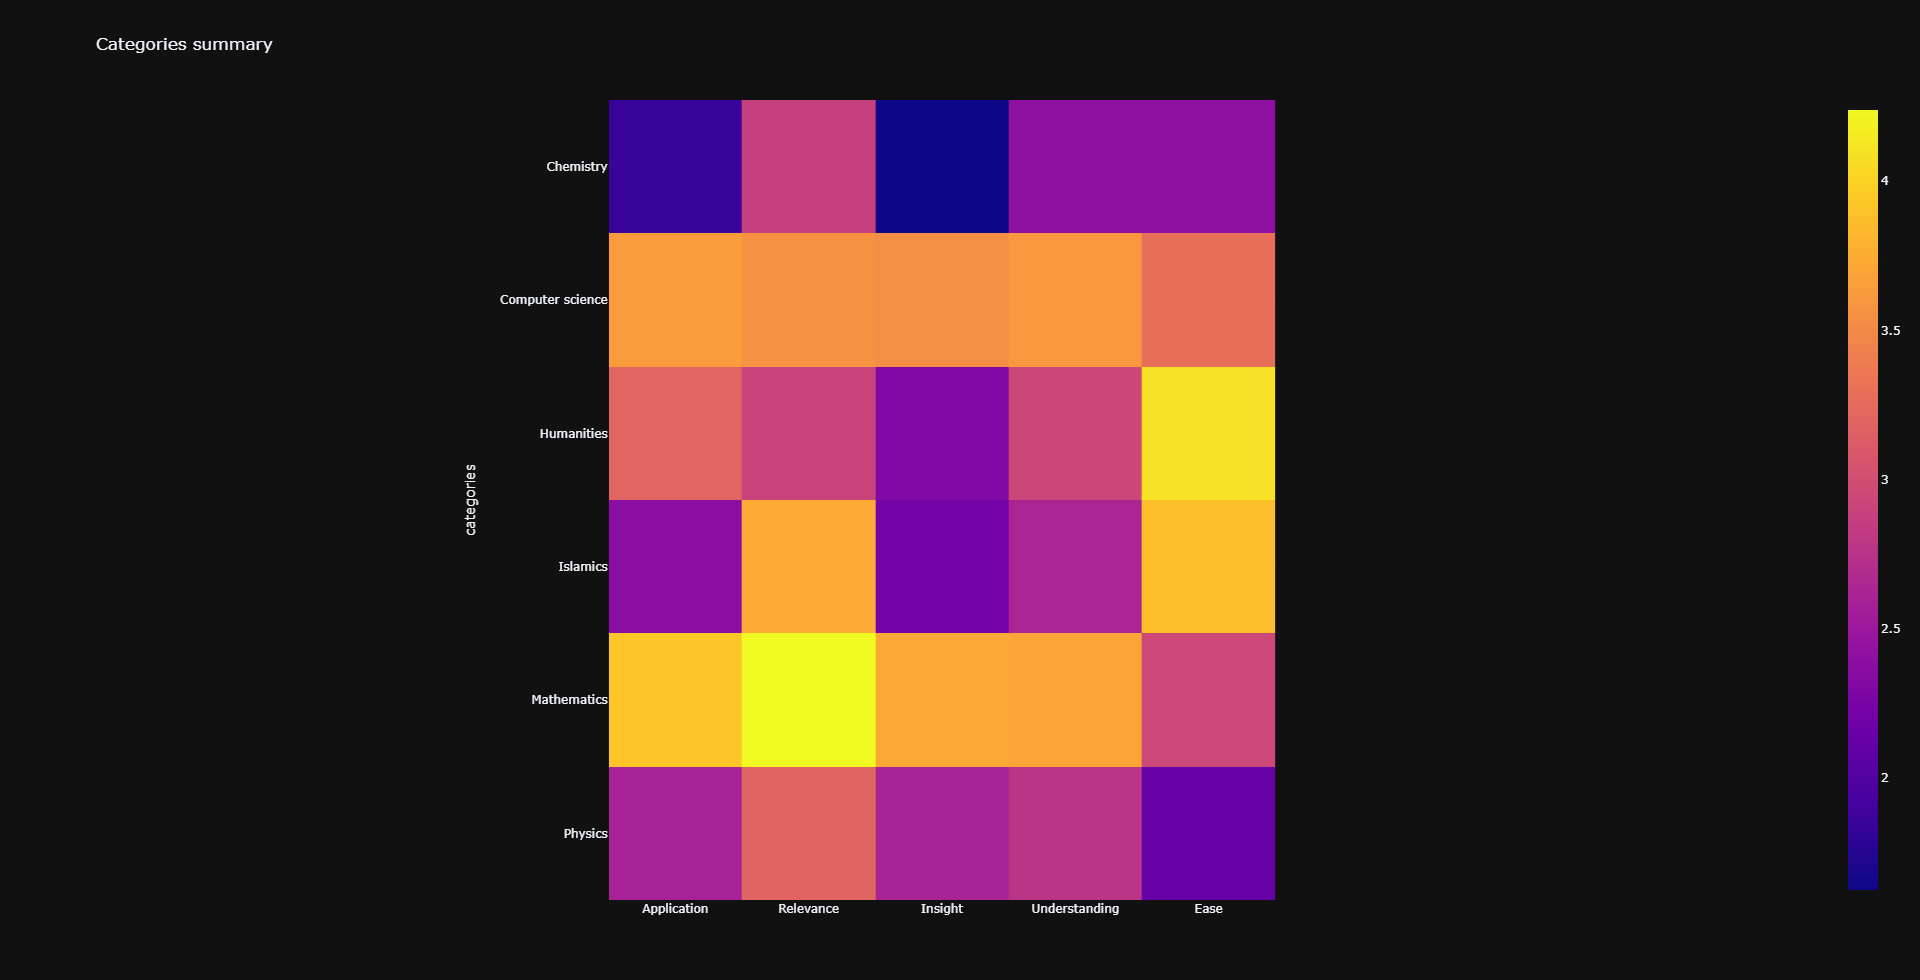
\includegraphics[scale=.3]{Categories summary.png}}
    \caption{Scores based on Real-world Vs. Academic ranking}
    \label{fig:my_label}
\end{figure}


\clearpage

\subsection{Observations}
We will detail a couple observations from the visualizations.

\paragraph{Figure \ref{fig:general_ranking}}
\begin{enumerate}
    \item The top three courses in general ranking are CSC311, CSC329 and CSC111. All of which are core computer science and are highly applicable.
    \item The bottom three courses in general ranking are CHEM101, PHYS104 and SALAM108. All of which are not computer science related, and are all studied in high school already.
    \item The lowest ranking Math courses are MATH106 and MATH244, probably due to it's unrelated nature compared to other math courses like MATH281 and MATH151 as well as being harder than all math courses.
    \item The lowest ranking computer science course is unsurprisingly CSC343 (Intro to Software Engineering).
\end{enumerate}

\paragraph{Figure \ref{fig:real_vs_academic}}
\begin{enumerate}
    \item We can see a general linear pattern in the scatter plot, which tells us that having a high academic score is intimately correlated with having a high real-world score.
    \item Outliers which have a high Academic score but a low Real-world score are CSC339 (Theory of computation) and CSC340 (Compilers and translation).
    \item Outliers which have a high Real-world score but a low Academic score are the two English courses, which makes sense, as English is extremely useful in the real world, but isn't academically related to computer science.
\end{enumerate}

\paragraph{Figure \ref{fig:my_label}}
\begin{enumerate}
    \item Computer science and Mathematics categories are highly correlated in all criteria, though we can see that mathematics have a higher score in relevance but a lower score in Ease. This makes sense if one considers that math is slowly changing, and courses like calculus are up to date, where courses like CSC453 (Parallel processing) and CSC380 (Databases) have developed so much compared to how they're studied in class.
    \item Humanities are generally easy, un-Insightful and its content is not up to date, similar to Islamics, with the exception of Relevance.
    \item Chemistry has extremely low values for all criteria, probably because the category is very distant from computer science and the category has only one course in it.
\end{enumerate}

\section{Conclusion}
After looking at student opinions on all courses, we compiled a number of suggestions to alter the computer science plan in hopes of raising the scores.

\paragraph{Low Relevance scores}
A few courses had excessively low Relevance scores, this means students think these courses are very old and need updating. Courses under 3 in relevance are:
\begin{enumerate}
    \item ARB100
    \item TECH101\footnote{This course has been overhauled recently, and most reviewers have not studied the overhauled course}
    \item Entrepeneure101.
    \item FAJAB101
    \item NAHAJ
    \item CHEM101
    \item CSC380
    \item CSC343
    \item CSC453
    \item CSC443
\end{enumerate}

Low relevance score in core computer science courses like CSC380 and CSC453 is not good, and an easy way to improve those courses is by updating the material. CSC380 for instance is only concerened with relational databases, where in the real world so many database variants are out there but the course doesn't even mention them as it created ages ago.

\paragraph{High Application scores}
The highest computer science Application scores are doing something right, we will mention their names and detail what those courses do differently from other courses.
\begin{enumerate}
    \item CSC111 (Programming I)
    \item CSC212 (Data Structures)
    \item CSC311 (Algorithm analysis and design)
    \item CSC462 (Machine learning)
\end{enumerate}
All courses mentioned had many Labs/Homeworks/Programming Assignments, other courses with very low application scores had relatively few or no programming assignments, thus, we can see that this factor is highly correlated with the application score. This doesn't mean imposing assignments on courses like CSC304 (Ethics) is going to be helpful though.

\paragraph{Low Understanding scores}
Many courses have low Understanding scores (i.e. rely heavily on memorization) such as:
\begin{enumerate}
    \item CSC343 (Intro to Software Engineering)
    \item CSC227 (OS)
    \item CSC443 (IT Project Management)
\end{enumerate}
This is not entirely due to the course's nature, as courses like Networking which have a large theoretical body to read scored very highly on this criterion. Carefully chosen questions on exams and quizzes can change the perception from memorization to understanding. This is generally unfavorable in all circumstances and is possibly an area where change could improve the computer science plan.



\subsection{Code \& Demo}
The code can be found at \href{https://github.com/Hawzen/Course-Ranking}{github.com/Hawzen/Course-Ranking} \\
A live demo can be found at \href{http://courses.hawzen.me}{courses.hawzen.me}.

\end{document}
